\chapter{Literature Survey}
% \begin{table}
% \begin{center}
% \begin{tabular}{|p{3cm}|p{3cm}|p{2cm}|p{4cm}|p{3cm}|}
% \hline
% \textbf{Title} & \textbf{Methodology} & \textbf{Results} & \textbf{Merits}  & \textbf{Demerits}\\
% \hline
% Violence detection using Oriented Violent Flows, 2016 [1] & AdaBoost and SVM classifier. & 88.00 percent & Feature representation model, which depicts the information involving both the motion magnitude and motion orientation. & Detection point where the behaviour is changing from normal to abnormal is time consuming.\\
% \hline
% Violent Flows:Real-Time Detection of Violent Crowd Behaviour, 2012 [2] & Global descriptors and SVM classifier & 5-fold cross validation: 81.30 percent & The algorithm detected far more violent scenes correctly, compared to existing work. It was furthermore far faster to detect the violence, typically in less than a second from its outbreak & Only magnitude of the flow vectors is considered, but the direction is not.\\
% \hline

% Automatic Fight
% Detection in
% Surveillance
% Videos, 2016 [3] & 
% Motion magnitude,
% motion acceleration
% and strength of
% motion region
% relationship,
% collectively known as
% motion signals & 
% 10 fold cross
% validation:
% 82.70 percent & 
% Difference
% between
% stimulated
% fights and real
% fights.
% Doesn’t rely
% on high level
% behaviour
% recognition,
% Thus applicable to Low quality videos. & 
%  Less accuracy is
% achieved when
% testing with real
% fight scenarios\\
% \hline

% Online real-time
% crowd behaviour
% detection in video
% sequences, 2015 [4] & 
% Instant entropy and
% temporal occupancy
% variation & 
% 96 percent
% Works
% without the
% need of
% training phase. &
% Computational
% speed (FPS) is
% varying for
% different
% datasets.\\
% \hline
% \end{tabular}
% \end{center}
% \caption{Literature Survey}
% \end{table}

\section{What is a video}
Video is a sequence of frames that has fixed frame width and height throughout its duration.
Video is an electronic medium for the recording, copying, playback,
broadcasting, and display of moving visual media.\par
Video was first developed for mechanical television systems, which were
quickly replaced by cathode ray tube (CRT) systems which were later replaced by flat
panel displays of several types. Video systems vary in display resolution, aspect ratio,
refresh rate, color capabilities and other qualities. Analog and digital variants exist and
can be carried on a variety of media, including radio broadcast, magnetic tape, optical
discs, computer files, and network streaming.

\section{What is Video Processing}
In electronics engineering, video processing is a particular case of signal
processing, which often employs video filters and where the input and output signals are
video files or video streams. \par Video processing techniques are used in television sets,
VCRs, DVDs, video codecs, video players, video scalers and other devices. For
example—commonly only design and video processing is different in TV sets of
different manufactures.

\section{Analysis of Crowd}
Crowd analysis involves the interpretation of data gained studying the natural
movement of groups or objects. Masses of bodies, particularly humans, are the subjects
of these crowd tracking analyses that include how a particular crowd moves and when a
movement pattern changes. The data is implemented in order to predict future crowd
movement, crowd density, and potential events such as an evacuation route.
Applications of crowd analysis can range from video game crowd simulation to security
and surveillance.
\par
Due to population growth, crowd analysis has become a major interest in social
and technical disciplines. Crowd analysis is being used to develop crowd management
strategies in public events as well as public space design, visual surveillance and virtual
environments to make areas more convenient in order to prevent crowd induced
disasters.
\subsection{What is crowd}
A crowd is a large group of people that are gathered or considered together. The
term "the crowd" may sometimes refer to the lower orders of people in general (the
mob). A crowd may be definable through a common purpose or set of emotions, such as
at a political rally, a sports event, or during looting (this is known as a psychological
crowd), or may simply be made up of many people going about their business in a busy
area.\par
The term crowd is sometimes defined in contrast to other group nouns for
collections of humans or animals, such as aggregation, audience, group, mass, mob,
populous, public, rabble and throng. Opinion researcher Vincent Price compares masses
and crowds, saying that "Crowds are defined by their shared emotional experiences, but
masses are defined by their interpersonal isolation."
\subsection{Challenges faced in crowd behaviour analysis}
Crowd analysis is a critical problem in understanding crowd behavior for
surveillance applications. The current practice is manually scanning video feeds from
several sources. Video analytics allows the automatic detection of events of interest, but
it faces many challenges because of non-rigid crowd motions and occlusions.\par
Video analysis and scene understanding usually involve object detection,
tracking and behavior recognition. For crowded scenes, due to extreme clutters, severe
occlusions and ambiguities, the conventional methods without special considerations are
not appropriate. As Ali pointed out , the mechanics of human crowds are complex as a
crowd exhibits both dynamics and psychological characteristics, which are often goal
directed. This makes it very challenging to figure out an appropriate level of granularity
to model the dynamics of a crowd. Another challenge in crowded scene analysis is that
the specific crowd behaviors needed to be detected and classified may be both rare and
subtle , and in most surveillance scenarios, these behaviors have few examples to learn.
The problem of occlusion is one of the main reasons why computer vision is
hard in general. Specifically, this is much more problematic in Object Tracking.
Occlusion means that there is something you want to see, but can't due to some property
of your sensor setup, or some event. For tasks which tracks objects (people, cars, ...)
then occlusion occurs if an object that is being tracked is hidden (occluded) by another
object. Like two persons walking past each other, or a car that drives under a bridge.
The problem in this case is what you do when an object disappears and reappears again.
\begin{figure}[H]
\centering
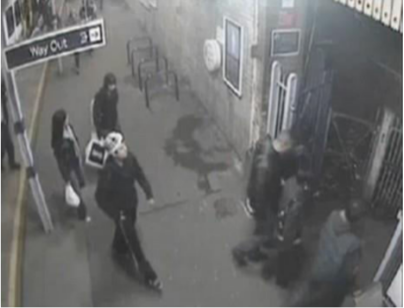
\includegraphics[scale = 0.6]{occlusion.png}
\caption{Occlusion Problem}
\end{figure}
Crowd scenes contain some uncertainities such as change of density, shape,
boundaries of the crowd. They do not define how to behave or share clear expectations
14on what will happen. They often feel something must be done right away to address
their common concern. Attitudes and ideas about the common concern spread very
quickly among crowd members. They often do and say things that they would normally
not do, and they go along with the actions of others in the crowd.\par
Certain crowd behaviours are normal in one scenario but may become hazards in
another. For example if we consider the running activity, running in a marathon can be
considered as a normal crowd behaviour but whereas running in a shopping mall or any
such rare places can be considered as an abnormal behaviour.
\begin{figure}[H]
\centering
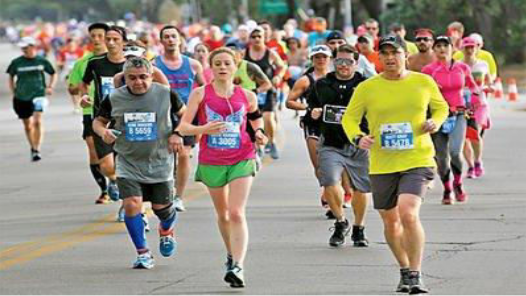
\includegraphics[scale = 0.7]{crowd_marathon.png}
\caption{Crowd Running in Marathon}
\end{figure}
\begin{figure}[H]
\centering
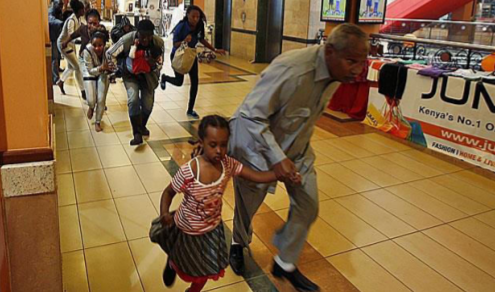
\includegraphics[scale = 0.7]{crowd_panic_mall.png}
\caption{Crowd Running in a Mall}
\end{figure}
\section{Optical Flow}
\subsection{What is Optical Flow}
Optical flow or optic flow is the pattern of apparent motion of objects, surfaces,
and edges in a visual scene caused by the relative motion between an observer and a
scene. The concept of optical flow was introduced by the American psychologist James
J. Gibson in the 1940s to describe the visual stimulus provided to animals moving
through the world. Gibson stressed the importance of optic flow for affordance
perception, the ability to discern possibilities for action within the environment.\par
Followers of Gibson and his ecological approach to psychology have further demonstrated the role of the optical flow stimulus for the perception of movement by
the observer in the world; perception of the shape, distance and movement of objects in
the world; and the control of locomotion.
The term optical flow is also used by roboticists, encompassing related
techniques from image processing and control of navigation including motion detection,
object segmentation, time-to-contact information, focus of expansion calculations,
luminance, motion compensated encoding, and stereo disparity measurement.

\subsection{Estimation}
Sequences of ordered images allow the estimation of motion as either
instantaneous image velocities or discrete image displacements. Fleet and Weiss
provide a tutorial introduction to gradient based optical flow. John L. Barron, David J.
Fleet, and Steven Beauchemin provide a performance analysis of a number of optical
flow techniques. It emphasizes the accuracy and density of measurements.\par
The optical flow methods try to calculate the motion between two image frames
which are taken at consecutive time frames at every voxel position. These methods are
called differential since they are based on local Taylor series approximations of the
image signal; that is, they use partial derivatives with respect to the spatial and temporal
coordinates. \par
For a 2D+t dimensional case (3D or n-D cases are similar) a voxel at location (x,y,t)
with intensity I(x,y,t) will have moved between the two image frames, and the following
brightness constancy constraint can be given:
\begin{equation}
I(x,y,t) = T(x + \Delta x, y + \Delta y, t + \Delta t)
\end{equation}
\begin{equation}
\frac{\partial I}{\partial x}V_x + \frac{\partial I}{\partial y}V_y + \frac{\partial I}{\partial t} = 0
\end{equation}